\documentclass{lab}

\begin{document}

\labtitle{4.7.2}{Эффект Поккельса}{7~февраля~2019~г.}{14~февраля~2019~г.}

\section*{Постановка эксперимента}

\begin{quote}
	\textbf{{\normalsize Цель работы: }}
	исследовать интерференцию рассеянного света, прошедшего кристалл; наблюдать изменения 
	характера поляризации света при наложении на кристалл электрического поля.
\end{quote}

\begin{quote}
	\textbf{{\normalsize Оборудование: }}
	гелий-неоновый лазер, поляризатор, кристалл ниобата лития, матовая пластина, экран, 
	источник высоковольтного переменного и постоянного напряжения, фотодиод, осциллограф, 
	линейка.
\end{quote}

\subsection*{Теоретическая часть}

Эффектом Поккельса называется изменение показателя преломления света в кристалле под действием 
электрического поля, причем это изменение пропорционально напряженности электрического поля. 
Как следствие эффекта Поккельса в кристалле появляется двойное лучепреломление или меняется 
его величина, если кристалл был двулучепреломляющим в отсутствие поля.\\

В нашем опыте используется поперечный электрооптический эффект. Исследуемый кристалл -- ниобат 
лития $ (LiNbO_3) $ -- является одноосным кристаллом, оптические свойства которого обладают 
симметрией вращения относительно некоторого одного направления, называемого \textit{оптической 
осью} $ Z $ кристалла.

Для световой волны, вектор $ \vec{E} $ которого перпендикулярен оси $ Z $, показатель 
преломления равен $ n_o $, а для волны с $ \vec{E} $ вдоль оси $ Z $ он равен $ n_e $ $ n_e < 
n_o $.

В общем случае, когда луч света распространяется под углом $ \Theta $ к оси~$ Z 
$~(рис.~\ref{setup}), существует два собственных значения показателя преломления $ n_1 $ и $ 
n_2 $: если $ \vec{E} \perp (\vec{k}, \vec{Z})$, где $ \vec{k} $ -- волновой вектор луча, то 
волна называется \textit{обыкновенной} (ординарной), а показатель преломления $ n_1 $ равен $ 
n_o $ и не зависит от угла $ \Theta $; когда $ \vec{E} \in (\vec{k}, \vec{Z}) $ -- это 
\textit{необыкновенная} (экстраординарная) волна, при этом показатель преломления $ n_2 $ 
зависит от угла $ \Theta $:
$$ \frac{1}{n_2^2} = \frac{\cos^2\Theta}{n_o^2} + \frac{\sin^2\Theta}{n_e^2} $$

Расположим перед кристаллом матовою пластину для рассеивания луча. Тогда на экране за поляроидом мы увидим концентрические кольца. При интерференции разность фаз обыкновенной и необыкновенной волнами, при прохождении через кристалл длиной $ l $, равна:
\begin{equation}\label{eq_1}
\Delta\varphi = \frac{2\pi}{\lambda} \cdot l \cdot (n_1 - n_2)
\end{equation}

\begin{figure}[H]
	\centering
	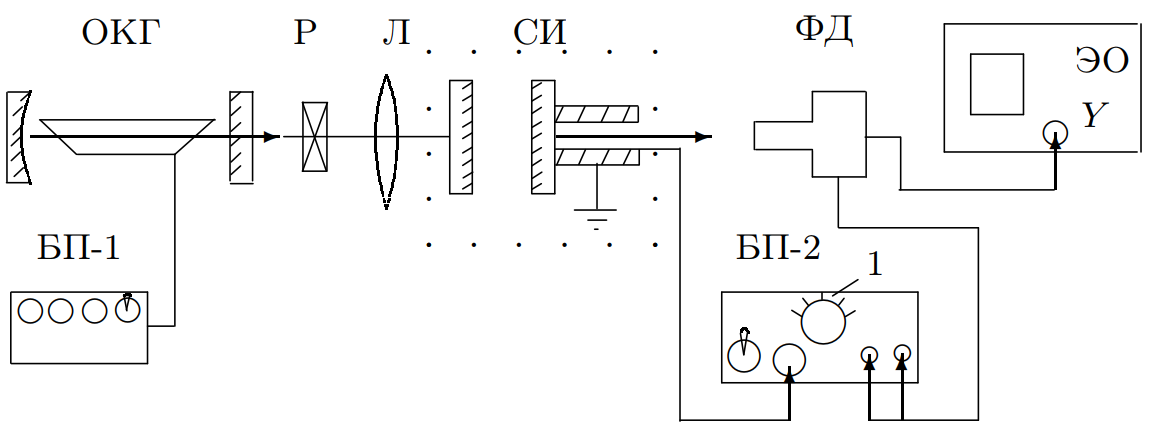
\includegraphics[width = 0.7 \textwidth]{setup}
	\caption{Схема установки для исследования эффекта Поккельса.}
	\label{setup}
\end{figure}

Для обыкновенного луча $ n_1 = n_o $ и не зависит от угла $ \Theta $. Для необыкновенного луча $ n_2 $ зависит от угла $ \Theta $ и определяется уравнением~\eqref{eq_1}. В силу малости углов $ (\sin\Theta\approx\Theta; \cos\Theta\approx 1 - \Theta^2/2) $ получаем $ n_2 = n_o - (n_o - n_e) \Theta^2 $.
$$ \delta = \frac{2\pi}{\lambda}\cdot l(n_o - n_e)\Theta^2 $$

Направления постоянной фазы -- конусы $ \Theta = const $. Будем нумеровать кольца итератором $ m $. Для $ m $-го темного кольца $ \delta = 2 \pi m $ или $ \delta = 2\pi \cdot l(n_o - n_e) \Theta^2 / \lambda = 2 \pi m $. Если $ L $ -- расстояние от центра кристалла до экрана, то, учитывая з-н Снеллиуса, при $ \Theta_{внешн} = n_o \Theta $ радиус кольца:
\begin{equation}\label{eq_2}
r_m^2 = \frac{\lambda}{l} \frac{(n_oL)^2}{(n_o-n_e)}m
\end{equation}

\begin{wrapfigure}{r}{5cm}
	\vspace{-2cm}
	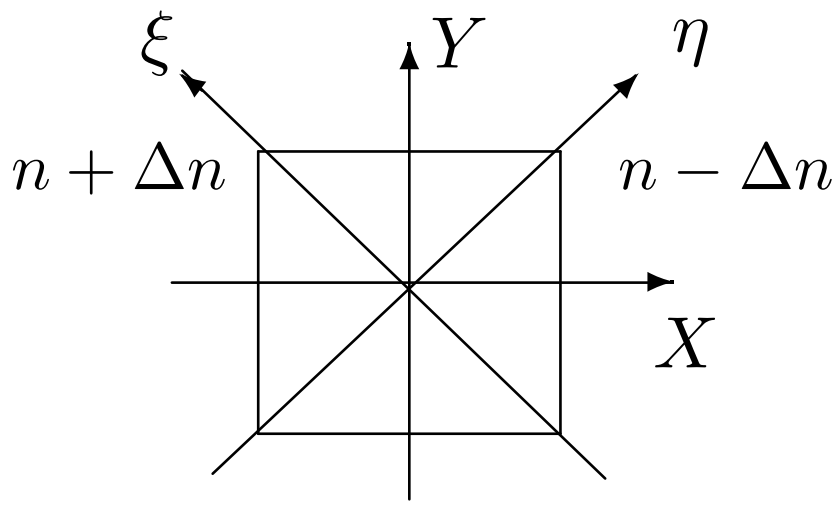
\includegraphics[width=5cm]{crystal}
	\caption{Появление новых главных направлений при наложении электрического поля.}
	\label{crystal}
\end{wrapfigure}

Остюда найдем $ (n_o - n_e) $ -- двулучепреломление кристалла. Разложим $ E = E_0e^{i(\omega t-kz)} $ по осям $ \xi $ и $ \eta $ (рис. \ref{crystal}). Появится разность фаз:
$$ \delta = \frac{2 \pi l}{\lambda}2\Delta n = \frac{4 \pi l}{\lambda}AE_{эл} = \frac{4\pi}{\lambda}\frac{l}{d}AU $$

$ U = E_{эл} \cdot d $ -- напряжение на кристалле, $ d $ -- размер кристалла в поперечном направлении. На направление $ X $ на выходе:
$$ E_{вых} = \frac{E_0}{2}e^{i(\omega t - kl)}(e^{i\delta/2} - e^{-i\delta/2}) = E_0 e^{i(\omega t - kl)} \sin \left(\frac{\delta}{2}\right) $$

Интенсивность света пропорциональна квадрату модуля вектора электрического поля в волне:
$$ I_{вых} \sim EE^* = E_0^2\sin^2\left(\frac{\delta}{2}\right) $$
\begin{equation}\label{eq_3}
I_{вых} = I_0 \sin^2\left(\frac{\delta}{2}\right) = I_0\sin^2\left(\frac{\pi}{2} \frac{U}{U_{\lambda/2}}\right)
\end{equation}
\begin{equation}\label{eq_4}
U_{\lambda/2} = \frac{\lambda}{4A}\frac{d}{l}
\end{equation}
-- так называемое \textit{полуволновое напряжение}: при $ U = U_{\lambda/2} $ сдвиг фаз между двумя волнами, соответствующими двум собственным поляризациям, $ \delta = \pi $ (разность хода равна $ \lambda/2 $), и интенсивность света на выходе анализатора достигает максимума.

При параллельных поляризациях лазера и анализатора:
\begin{equation}\label{eq_5}
I_{вых} = I_0\cos^2\left(\frac{\pi}{2}\frac{U}{U_{\lambda/2}}\right)
\end{equation}
\begin{figure}[H]
	\centering
	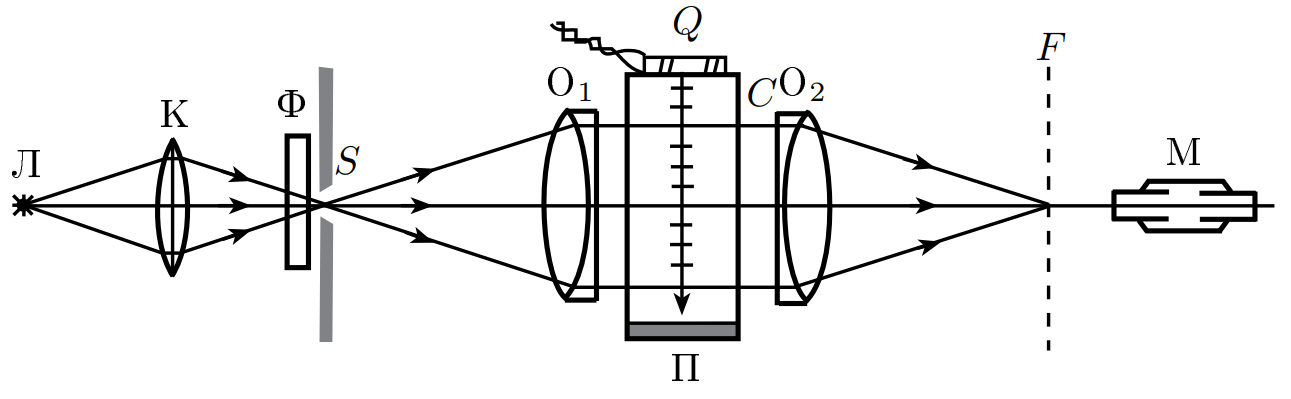
\includegraphics[width = 0.5 \textwidth]{scheme}
	\caption{Схема для изучения двойного лучепреломления в электрическом поле.}
	\label{scheme}
\end{figure}

\section*{Выполнение эксперимента}

Кристалл ниобата лития имеет размеры: $ 3 \times 3 \times 26~мм $. Волна гелий-неонового лазера: $ \lambda = 0.63~мкм $ в ниобате лития $ n_o = 2.29 $.

$ n_o = \sqrt{\varepsilon_{\perp}} $ -- у обыкновенной волны;

$ n_e = \sqrt{\varepsilon_{\parallel}} $ -- вдоль $ \vec{k} $.

\begin{enumerate}
\item
Установим кристалл на расстоянии $ L = (87 \pm 1)~см $ от экран.

Снимем зависимость $ r^2(m) $, где радиус концентрических колец при скрещенной поляризации (таблица \ref{tab1}).

\begin{table}[H]
	\hspace{-1cm}
	\centering
	%\resizebox{\textwidth}{!}{
		\begin{tabular}{|c|ccccccccc|}
			\hline
			$m$			&1 &2 &3 &4 &5 &6 &7 &8 &9 \\
			$r,~мм$		&31 &44 &54 &63 &70 &77 &84 &89 &94 \\
			$r^2,~см^2$	&9.6 &19.4 &29.2 &39.7 &49.0 &59.3 &70.6 &79.2 &88.4 \\ \hline
		\end{tabular}
	%}
	\caption{Зависимость радиуса темных колец $ r(m) $ и $ r^2(m) $ от номера кольца $ m $.}
	\label{tab1}
\end{table}

\item
Построим график зависимости радиуса колец от их номера $ r^2 = f(m) $:

\begin{figure}[H]
	\centering
	\begin{tikzpicture}
	
	\pgfplotstableread{
		X	Y		x-err	y-err
		1	09.6		00		5
		2	19.4		00		5 
		3	29.2		00		5
		4	39.7		00		5
		5	49.0		00		5
		6	59.3		00		5
		7	70.6		00		5
		8	79.2		00		5
		9	88.4		00		5
	}{\mytable}
	
	\begin{axis}[
	width = 0.8\textwidth,
	grid = major,
	xlabel = $ m $,
	ylabel = $ r^2\text{, см}^2 $,
	xmin = 0,
	ymin = 0,
	xmax = 10,
	ymax = 100
	]
	
	\addplot[
	only marks,
	color = red,
	mark = *,
	error bars/.cd,
	x dir = both,
	x explicit,
	y dir = both,
	y explicit
	]
	table[
	x error = x-err,
	y error = y-err
	] {\mytable};
	
	\addplot[
	mark = none,
	color = red
	]
	table[
	y = {create col/linear regression={y=Y}}
	] % compute a linear regression from the
	{\mytable};
	
	\end{axis}
	\end{tikzpicture}
	\caption{Зависимость $ r^2=f(m) $.}
	\label{g_1}
\end{figure}

\item
Из графика (рис. \ref{g_1}) найдем:
$$ \tan \psi = (9.95 \pm 0.08),~\varepsilon \approx 1 \% $$
$$ \then (n_o - n_e) = \frac{\lambda}{l} \frac{(n_oL)^2}{\tan\psi} = (9.6 \pm 0.3) \cdot 10^{-2},~\varepsilon \approx 3 \% $$

\item
Рассмотрим минимумы и максимумы при различной поляризации и постоянным напряжении:

\begin{table}[H]
	\hspace{-1cm}
	\centering
	\begin{tabular}{|c|cr|cr|}
		\hline
		$Поляризация$	&\multicolumn{2}{c|}{Параллельно} &\multicolumn{2}{c|}{Перпендикулярно} \\
		$Минимумы, дел$	&31 &92 &60 &-~ \\
		$Максимумы, дел$&60 &-~ &30 &90 \\ \hline
	\end{tabular}
	\caption{Зависимость радиуса темных колец $ r(m) $ и $ r^2(m) $ от номера кольца $ m $.}
	\label{tab2}
\end{table}

\vspace{-0.5cm}

\item
Из таблицы \ref{tab2} найдем: $ U_{\lambda/2} = 30~дел~= 450~В $.

\item
Аналогично найдем $ U_{\lambda/2} $ при помощи переменного напряжения по изображениям на экране осциллографа: $ U_{\lambda/2} \approx 30~дел~\approx 450~В $.

\item
Приведем изображения экрана осциллографа при $ U_{\lambda/2}, U_{\lambda}, U_{3\lambda/2} $ при различных поляризациях (рис. \ref{image}):
\begin{figure}[H]
	\begin{center}
		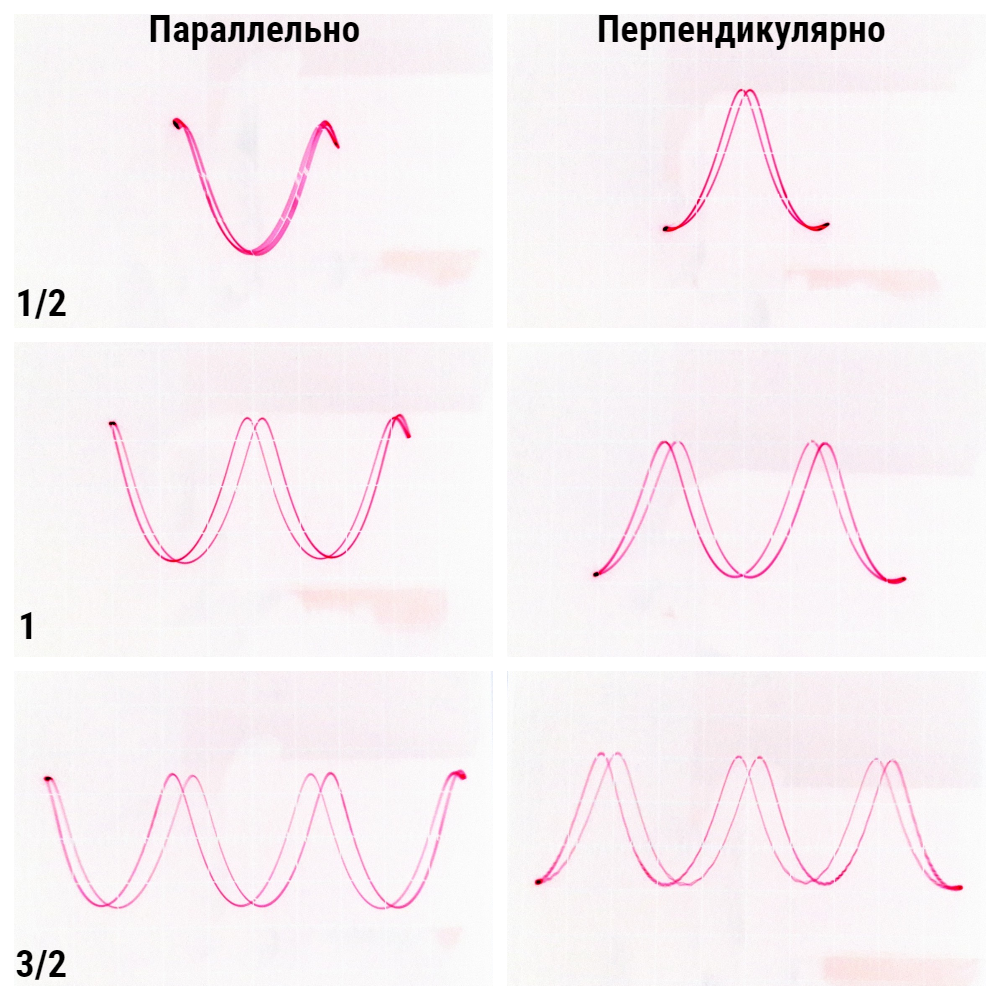
\includegraphics[width = 0.7 \textwidth]{image}
		\caption{Фигуры Лиссажу при различных значениях напряжений и поляризациях.}
		\label{image}
	\end{center}
\end{figure}

\end{enumerate}

\vspace{-1.5cm}

\section*{Итоги}

В эксперименте наблюдался эффект Поккельса -- изменение показателя преломления света в кристалле под действием внешнего электрического поля, причем было установлено, что данное изменение пропорционально напряженности электрического поля.

Получено двулучепреломление: $ (n_o - n_e) = (9.6 \pm 0.3) \cdot 10^{-2},~\varepsilon \approx 3 \% $

Определено полуволновое напряжение: $ U_{\lambda/2} \approx 450~В $

\end{document}